\chapter{Resultados}

A partir dos resultados iniciais, desenvolveram-se mais e mais modificações para melhorá-los.

\section{Resultados preliminares}
Inicialmente, o número de Prandtl turbulento, $Pr_t = 0.71$, foi usado como o da literatura. Os resultados obtidos são mostrados na figura \ref{figuraresultados1} e comparados com DNS de (Kawamura, 2007) e (kasagi et al., 1992).\\
\begin{figure*}[h!] 
	\centering
	%		\begin{subfigure}[t]{0.49\textwidth}
	%		\centering
	%		\includegraphics[angle=0, scale=0.32]{fotos_formatacao_final/Temperature_150_0025_classico}
	%		\caption{Temperature configuration for $Re_\tau = 150$, $Pr = 0.025$, $L2 = 0.13$ }
	%		\end{subfigure}%
	\begin{subfigure}[t]{0.49\textwidth}
		\centering
		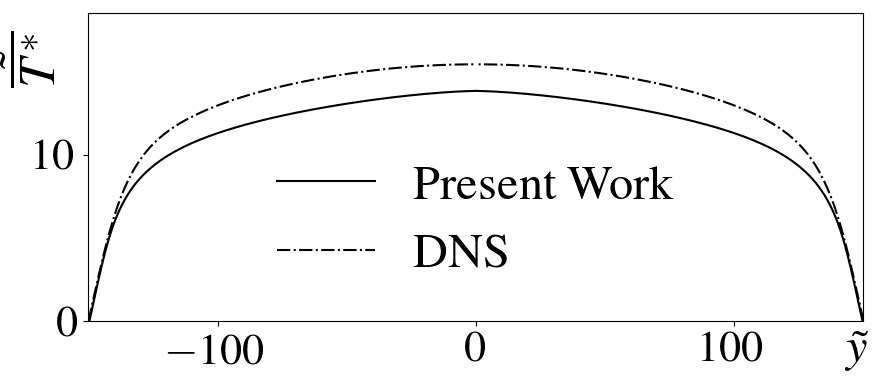
\includegraphics[angle=0, scale=0.24]{fotos_formatacao_final/Temperature_150_071_classico}
		\caption{Distribuição de temperatura para $Re_\tau = 150$, $L2 = 1.42$}
	\end{subfigure}
	%		\begin{subfigure}[t]{0.49\textwidth}
	%		\centering
	%		\includegraphics[angle=0, scale=0.32]{fotos_formatacao_final/Temperature_395_0025_classico}
	%		\caption{Temperature configuration for $Re_\tau = 395$, $Pr = 0.025$, $L2 = 0.52$}
	%		\end{subfigure}%
	\begin{subfigure}[t]{0.49\textwidth}
		\centering
		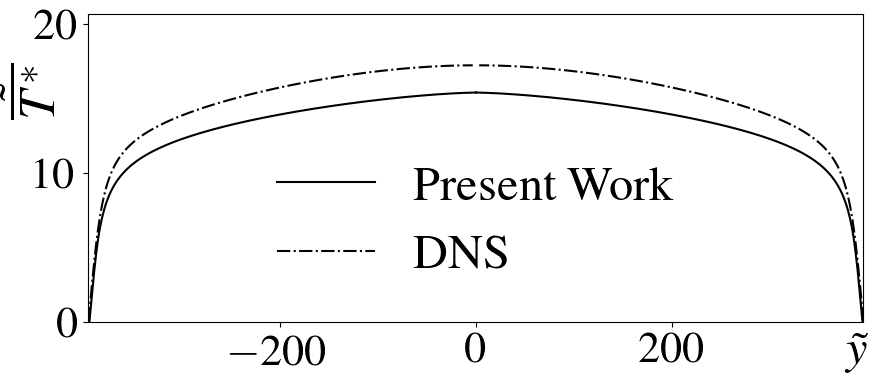
\includegraphics[angle=0, scale=0.24]{fotos_formatacao_final/Temperature_395_071_classico}
		\caption{Distribuição de temperatura para $Re_\tau = 395$, $L2 = 1.55$}
	\end{subfigure}
	%		\centering
	%		\begin{subfigure}[t]{0.49\textwidth}
	%		\centering
	%		\includegraphics[angle=0, scale=0.32]{fotos_formatacao_final/Temperature_395_1_classico}
	%		\caption{Temperature configuration for $Re_\tau = 395$, $Pr = 1.0$, $L2 = 1.89$}
	%		\end{subfigure}%
	%		\begin{subfigure}[t]{0.49\textwidth}
	%		\centering
	%		\includegraphics[angle=0, scale=0.32]{fotos_formatacao_final/Temperature_395_2_classico}
	%		\caption{Temperature configuration for $Re_\tau = 395$, $Pr = 2.0$, $L2 = 2.60$}
	%		\end{subfigure}\\
	%		\begin{subfigure}[t]{0.49\textwidth}
	%		\centering
	%		\includegraphics[angle=0, scale=0.32]{fotos_formatacao_final/Temperature_395_5_classico}
	%		\caption{Temperature configuration for $Re_\tau = 395$, $Pr = 5.0$, $L2 = 3.75$}
	%		\end{subfigure}%
	%		\begin{subfigure}[t]{0.49\textwidth}
	%		\centering
	%		\includegraphics[angle=0, scale=0.32]{fotos_formatacao_final/Temperature_395_7_classico}
	%		\caption{Temperature configuration for $Re_\tau = 395$, $Pr = 7.0$, $L2 = 4.24$}
	%		\end{subfigure}\\
	%	    \centering
	%		\begin{subfigure}[t]{0.49\textwidth}
	%		\centering
	%		\includegraphics[angle=0, scale=0.32]{fotos_formatacao_final/Temperature_395_10_classico}
	%		\caption{Temperature configuration for $Re_\tau = 395$, $Pr = 10.0$, $L2 = 4.55$}
	%		\end{subfigure}%
	%		\begin{subfigure}[t]{0.49\textwidth}
	%		\centering
	%		\includegraphics[angle=0, scale=0.32]{fotos_formatacao_final/Temperature_640_0025_classico}
	%		\caption{Temperature configuration for $Re_\tau = 640$, $Pr = 0.025$, $L2 = 0.84$}
	%		\end{subfigure}\\
	\begin{subfigure}[t]{0.49\textwidth}
		\centering
		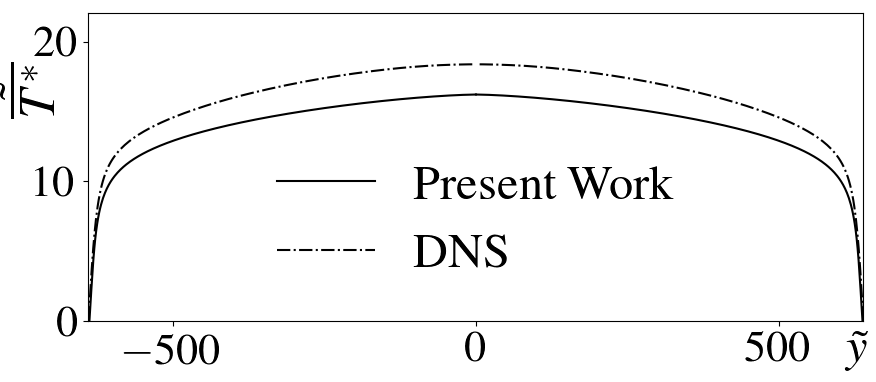
\includegraphics[angle=0, scale=0.24]{fotos_formatacao_final/Temperature_640_071_classico}
		\caption{Distribuição de temperatura para $Re_\tau = 640$, $L2 = 1.79$}
	\end{subfigure}%
	\begin{subfigure}[t]{0.49\textwidth}
		\centering
		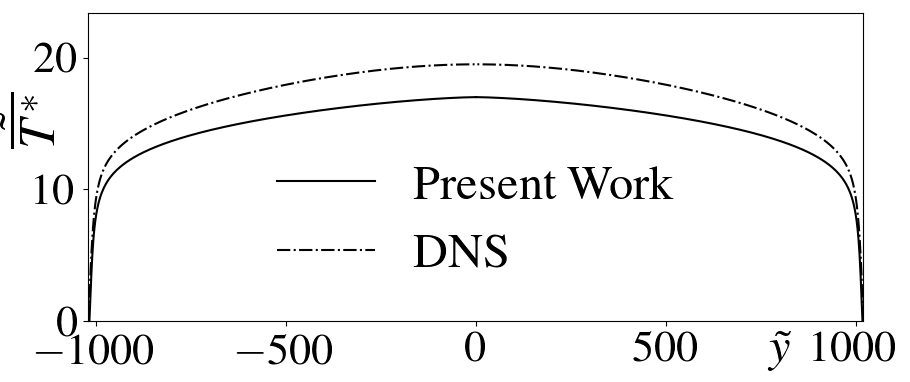
\includegraphics[angle=0, scale=0.24]{fotos_formatacao_final/Temperature_1000_071_classico}
		\caption{Distribuição de temperatura para $Re_\tau = 1020$, $L2 = 2.04$}
	\end{subfigure}%
	\caption{Distribuição de temperatura para $Pr_t = 0.71$, $A = 26$ e $Pr = 0.71$} 
	\label{figuraresultados1}
\end{figure*}	

Os primeiros resultados não foram satisfatórios. Então, notou-se que o número de Prandtl turbulento teve grande influência no resultado, então o número de Prandtl turbulento do DNS (figura \ref{figure5}) foi utilizado como parâmetro no programa, obtendo-se uma norma L2 de $ 0.19 $ para $ Re_t = 640 $. Assim, se observou que o problema se encontrava com a parametrização do número de Prandtl turbulento. Assim, este virou o foco da pesquisa.

\begin{figure*}[h!]
	\centering
	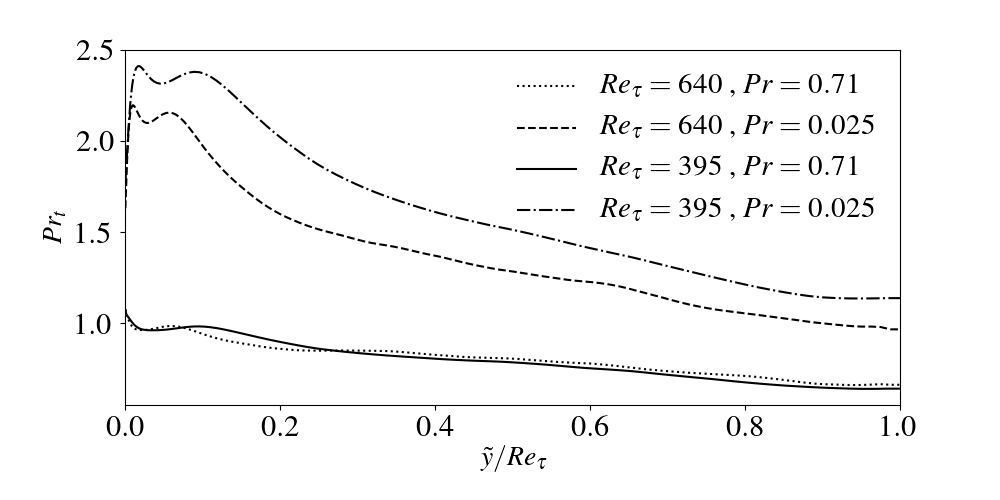
\includegraphics[angle=0, scale=0.4]{fotos_formatacao_final/DNS_PRt}
	\caption{Prandtl do DNS com o número de Prandtl turbulento de acordo com a coordenada $ y $ do canal.}
	\label{figure5}
\end{figure*}

Assim, iniciou-se o esforço para propor uma parametrização ajustada para o número de Prandtl turbulento.
Neste sentido tentou-se ajustar um valor para o qual o erro foi mínimo comparado com o DNS. Neste sentido, a metodologia do algoritmo de evolução diferencial foi aplicada.



\section{A meta-modelagem, com o algoritmo genético: Evolução Diferencial (DE)}
Utilizou-se um algoritmo que buscou um erro mínimo para a função dada, considerando o número de Prandtl turbulento como variável editável e o menor erro como padrão de interesse.
Foi obtido um número de Prandtl turbulento ideal de $ 0.9$ , para o número de Reynolds turbulento de $ 1020$.
\begin{figure}[!h]
	\centering
	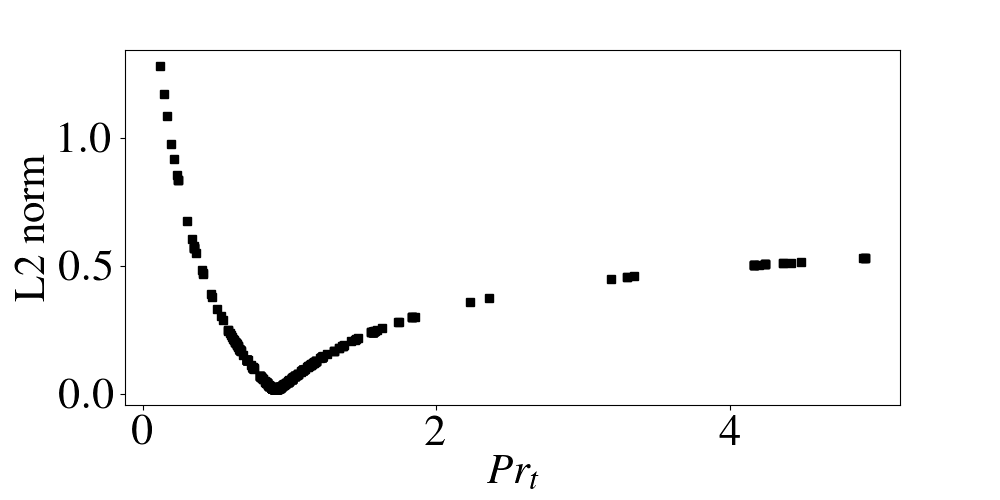
\includegraphics[angle=0, scale=0.31]{fotos_formatacao_final/Genetic_amostra}
	\caption{Iterações do algoritmo genético, com simulações para $Re_\tau = 1020$. Convergência em $Pr_t = 0.9 $.}
\end{figure}

O número de Prandtl turbulento obtido, $Pr_t = 0.9$, foi utilizado nos outros Reynolds turbulento, resultando em:
\begin{figure*}[!h]
	\centering
	\begin{subfigure}[t]{0.5\textwidth}
		\centering
		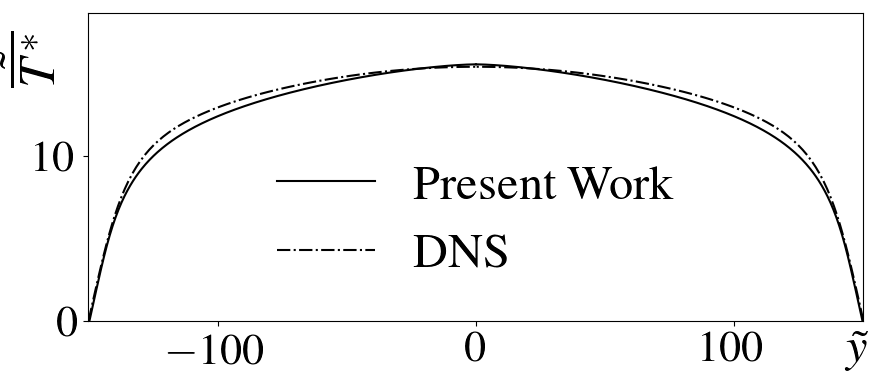
\includegraphics[angle=0, scale=0.24]{fotos_formatacao_final/Temperature_150_071_Prt0905_A26}
		\caption{Distribuição de temperatura para $Re_\tau = 150$, $L2 = 0.34$}
	\end{subfigure}
	\begin{subfigure}[t]{0.45\textwidth}
		\centering
		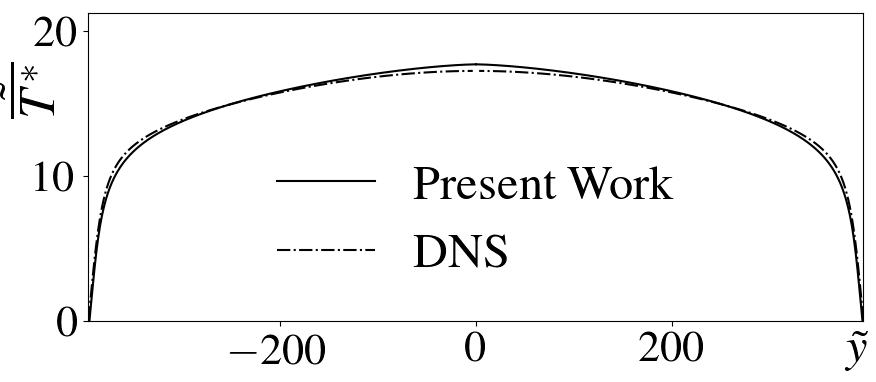
\includegraphics[angle=0, scale=0.24]{fotos_formatacao_final/Temperature_395_071_Prt0905_A26}
		\caption{Distribuição de temperatura para $Re_\tau = 395$, $L2 = 0.23$}
	\end{subfigure}
	\begin{subfigure}[t]{0.5\textwidth}
		\centering
		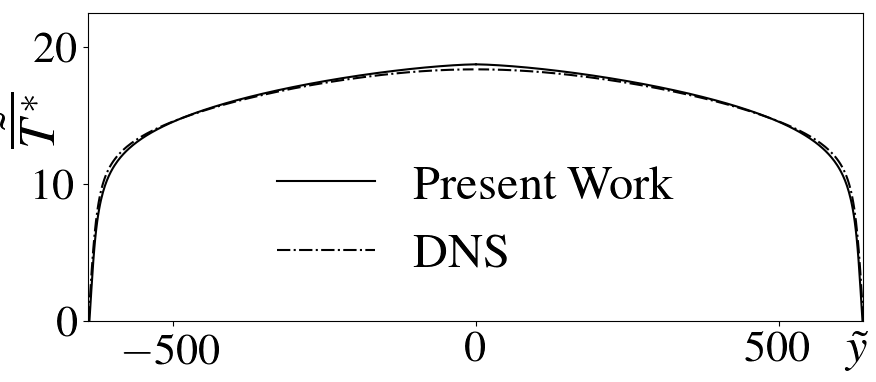
\includegraphics[angle=0, scale=0.24]{fotos_formatacao_final/Temperature_640_071_Prt0905_A26}
		\caption{Distribuição de temperatura para $Re_\tau = 640$, $L2 = 0.19$}
	\end{subfigure}
	\begin{subfigure}[t]{0.45\textwidth}
		\centering
		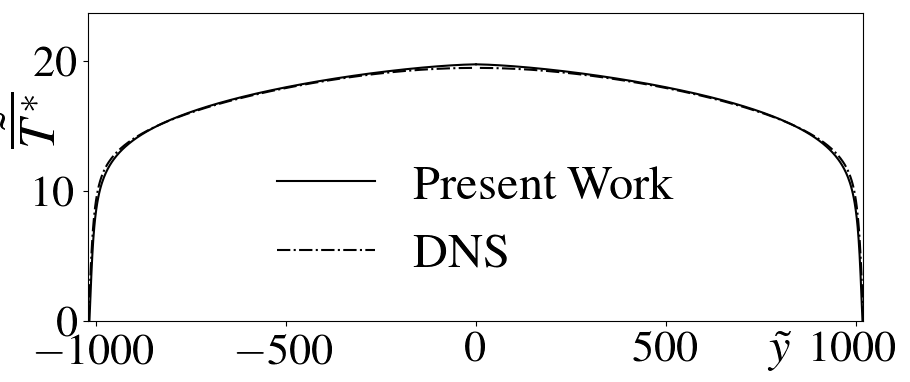
\includegraphics[angle=0, scale=0.24]{fotos_formatacao_final/Temperature_1000_071_Prt0905_A26}
		\caption{Distribuição de temperatura para $Re_\tau = 1020$, $L2 = 0.14$}
	\end{subfigure}	
	\caption{Resultado de simulações térmicas para $Pr_t = 0.9 $, $A = 26$ e $Pr =0.71$ }
\end{figure*}

Mesmo os resultados sendo muito melhores quando comparados ás figuras \ref{figuraresultados1}, o modelo tinha que ser melhorado. O número de Prandtl turbulento variava com o número de Reynolds turbulento, como visto em (fig.\ref{figure5}), assim, um modelo que contemplasse esse fato tinha de ser proposto. 
Para se obter uma curva para o $Pr_t$ em função de $Re_\tau$, o mesmo algoritmo de otimização teve que ser usado para determinar um número de Prandtl turbulento ideal para cada número de Reynolds turbulento disponível na base de dados de DNS. (Kawamura, 2007) e (kasagi et al., 1992).
Os melhores números de Prandtl turbulentos obtidos foram:

\begin{table}[!h]
	\centering
	\caption{Números de Prandtl turbulentos ideais ajustados para cada número de Reynolds turbulento, com $A = 26$}
	\begin{tabular}{ll}
		\hline
		$Re_\tau$ & $Pr_t$\\
		\hline
		150  &   0.94531\\
		395  &   0.89531\\
		640  &   0.89531\\
		1020 &   0.90000\\ 
		\hline
	\end{tabular}
\end{table}



Executando um ajuste de curva polinomial, um modelo ajustado para o número de Prandtl turbulento como uma função do número de Reynolds turbulento foi desenvolvido:
\begin{equation}
\begin{split}
Pr_t = -4.5604 * 10^{-10} Re_\tau^3 + 9.5690 * 10^{-7} Re_\tau^2 - 6.1715 *10 ^{-4} Re_\tau + 1.0178 
\end{split}
\end{equation}
Os resultados das simulações foram muito precisos, ainda mais do que as simulações com os números de Prandtl turbulentos definidos como os valores médios dos dos dados do DNS. (fig.\ref{figure5}). Estes foram:



\begin{figure*}[!h]
	\centering
	\begin{subfigure}[t]{0.5\textwidth}
		\centering
		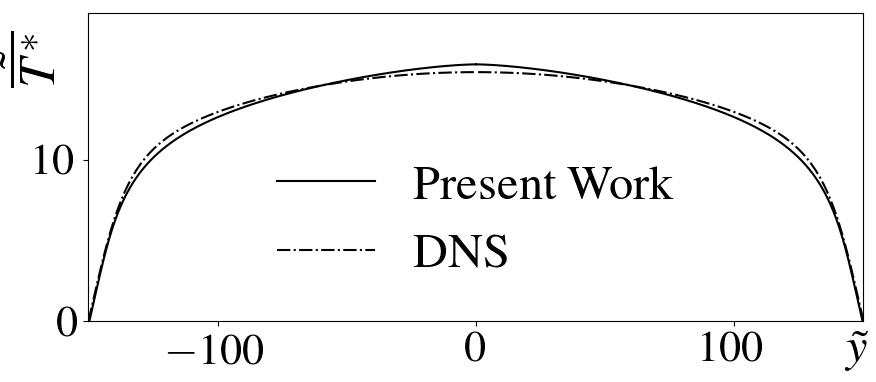
\includegraphics[angle=0, scale=0.24]{fotos_formatacao_final/Temperature_150_071_Prt(Ret)_A26}
		\caption{Distribuição de temperatura para $Re_\tau = 150$, $L2 = 0.26$}
	\end{subfigure}
	\begin{subfigure}[t]{0.45\textwidth}
		\centering
		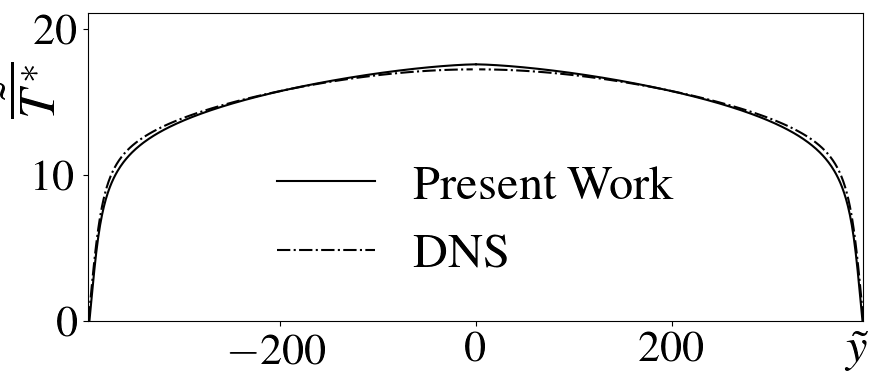
\includegraphics[angle=0, scale=0.24]{fotos_formatacao_final/Temperature_395_071_Prt(Ret)_A26}
		\caption{Distribuição de temperatura para $Re_\tau = 395$, $L2 = 0.22$}
	\end{subfigure}
	\begin{subfigure}[t]{0.5\textwidth}
		\centering
		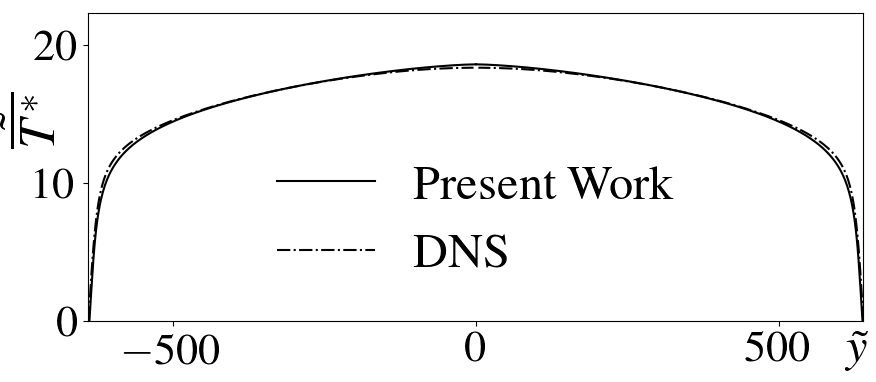
\includegraphics[angle=0, scale=0.24]{fotos_formatacao_final/Temperature_640_071_Prt(Ret)_A26}
		\caption{Distribuição de temperatura para $Re_\tau = 640$, $L2 = 0.17$}
	\end{subfigure}
	\begin{subfigure}[t]{0.45\textwidth}
		\centering
		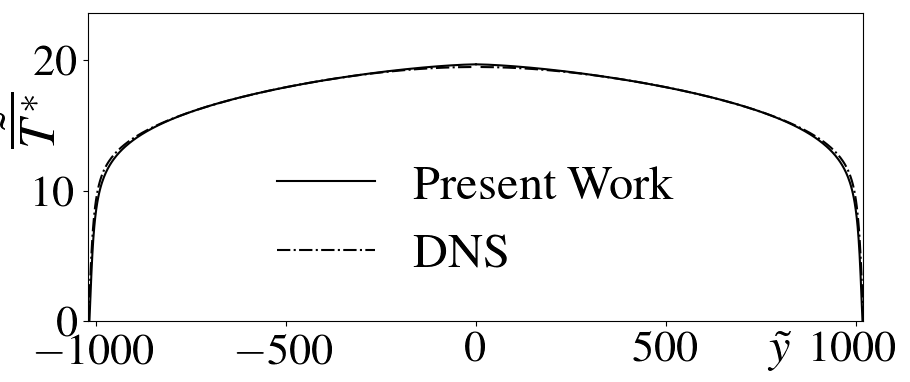
\includegraphics[angle=0, scale=0.24]{fotos_formatacao_final/Temperature_1000_071_Prt(Ret)_A26}
		\caption{Distribuição de temperatura para $Re_\tau = 1020$, $L2 = 0.14$}
	\end{subfigure}	
	\caption{Resultados de simulações térmicas para $Pr_\tau(Re_\tau)$, $A = 26$ e $Pr =0.71$ }
\end{figure*}



\newpage

Outras maneiras de reduzir a imprecisão foram pesquisadas. O perfil de velocidade foi uma possibilidade, uma vez que desempenha um papel importante no erro do método. Simulações foram realizadas desenvolvendo apenas essa propriedade física, e houve erro associado, como pode ser visto adiante:

\begin{figure*}[!h]
	\centering
	\begin{subfigure}[t]{0.5\textwidth}
		\centering
		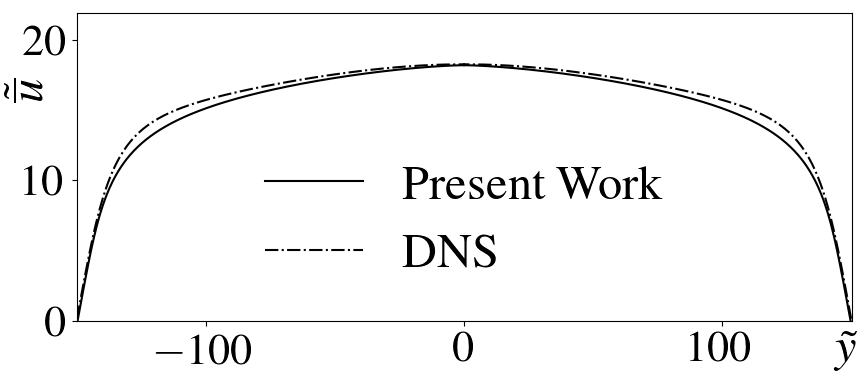
\includegraphics[angle=0, scale=0.24]{fotos_formatacao_final/Temperature_150_Avelocity}
		\caption{Distribuição de velocidade para $Re_\tau = 150$, $L2 = 0.47$}
	\end{subfigure}
	\begin{subfigure}[t]{0.45\textwidth}
		\centering
		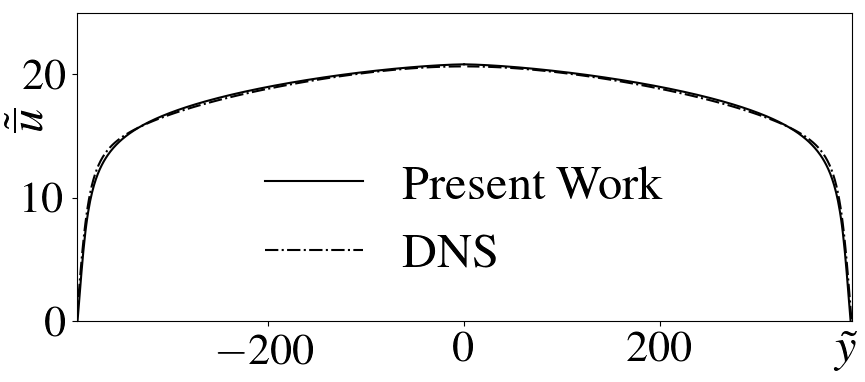
\includegraphics[angle=0, scale=0.24]{fotos_formatacao_final/Temperature_395_Avelocity}
		\caption{Distribuição de velocidade para $Re_\tau = 395$, $L2 = 0.17$}
	\end{subfigure}
	\begin{subfigure}[t]{0.5\textwidth}
		\centering
		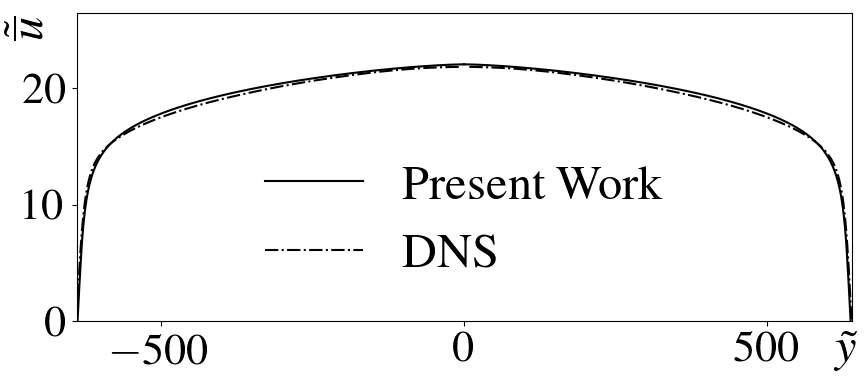
\includegraphics[angle=0, scale=0.24]{fotos_formatacao_final/Temperature_640_Avelocity}
		\caption{Distribuição de velocidade para $Re_\tau = 640$, $L2 = 0.23$}
	\end{subfigure}
	\begin{subfigure}[t]{0.45\textwidth}
		\centering
		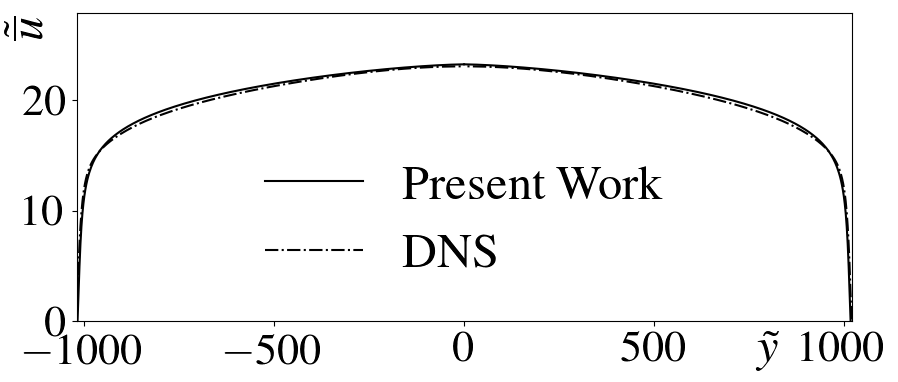
\includegraphics[angle=0, scale=0.24]{fotos_formatacao_final/Temperature_1000_Avelocity}
		\caption{Distribuição de velocidade para $Re_\tau = 1020$, $L2 = 0.23$}
	\end{subfigure}	
	\caption{Resultados de simulações dinâmicas para $A = 26$}
\end{figure*}

Um modelo ajustado foi preparado no presente trabalho para a constante de Cebeci $A$ com o objetivo de reduzir o erro e, por extensão, tornar o método mais preciso. O mesmo algoritmo usado para encontrar os números ideais de Prandtl turbulento foi usado para encontrar uma constante de Cebecis ideal para cada número de Reynolds turbulento. Foi utilizada a velocidade do DNS disponível para calcular a norma L2. A constante de Cebeci "A" foi definida como uma variável editável para o programa, e a norma L2 foi definida como um parâmetro de interesse. Os resultados para as constantes ideais do Cebeci podem ser vistos adiante:


\begin{table}[!h]
	\centering
	\caption{Constantes de Cebeci ideais ajustadas para cada Reynolds turbulento.}
	\begin{tabular}{ll}
		\hline
		$Re_\tau$ & $A$\\
		\hline
		150  &   28.616180\\
		395  &   25.673782\\
		640  &   25.001266\\
		1020 &   25.002136\\ 
		\hline
	\end{tabular}
	\label{tablea}
\end{table}

Dos pontos resultantes do algoritmo de otimização, um modelo de função de Cebeci fora ajustado:
\begin{equation}
A = \frac{Re_\tau ^{0.04510621 * \ln(Re_\tau)} *e ^ {5.27528132} }{Re_\tau ^{0.60941173}}
\end{equation}

Em seguida, foram feitas simulações com a função otimizada para um erro mínimo em relação à velocidade, como pode ser visto nas simulações, houve uma melhora nos resultados:


\begin{figure*}[!h]
	\centering
	\begin{subfigure}[t]{0.5\textwidth}
		\centering
		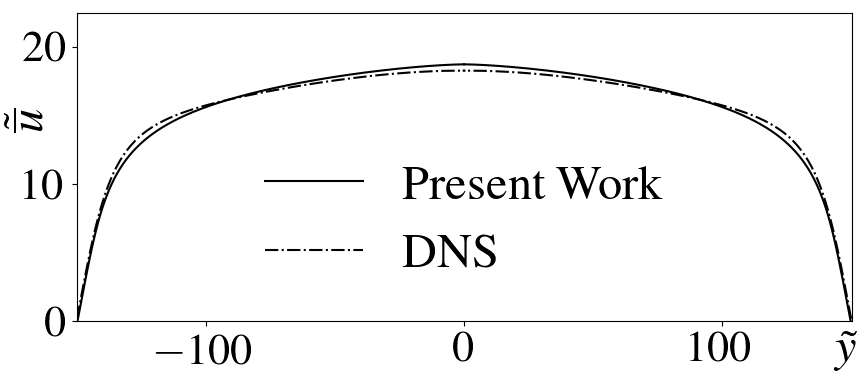
\includegraphics[angle=0, scale=0.24]{fotos_formatacao_final/Temperature_150_Amodeled}
		\caption{Distribuição de velocidade para $Re_\tau = 150$, $L2 = 0.28$}
	\end{subfigure}
	\begin{subfigure}[t]{0.45\textwidth}
		\centering
		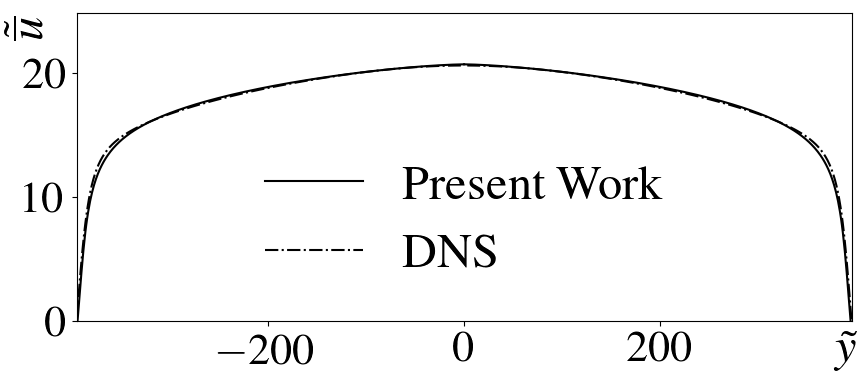
\includegraphics[angle=0, scale=0.24]{fotos_formatacao_final/Temperature_395_Amodeled}
		\caption{Distribuição de velocidade para $Re_\tau = 395$, $L2 = 0.16$}
	\end{subfigure}
	\begin{subfigure}[t]{0.5\textwidth}
		\centering
		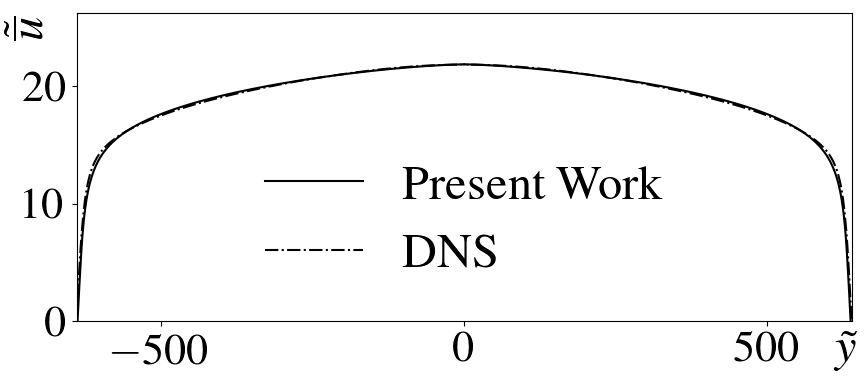
\includegraphics[angle=0, scale=0.24]{fotos_formatacao_final/Temperature_640_Amodeled}
		\caption{Distribuição de velocidade para $Re_\tau = 640$, $L2 = 0.14$}
	\end{subfigure}
	\begin{subfigure}[t]{0.45\textwidth}
		\centering
		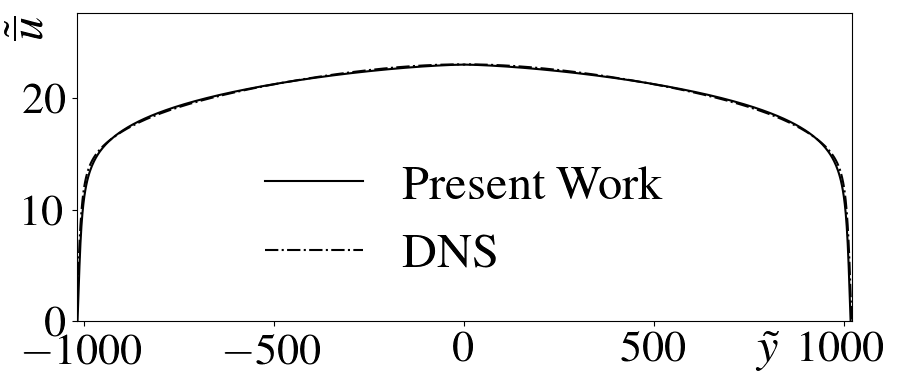
\includegraphics[angle=0, scale=0.24]{fotos_formatacao_final/Temperature_1000_Amodeled}
		\caption{Distribuição de velocidade para $Re_\tau = 1020$, $L2 = 0.13$}
	\end{subfigure}	
	\caption{Resultados para a velocidade com o valor de Cebeci modelado.}
\end{figure*}

Com a função do Cebeci ajustada, um novo grupo de otimizações foi feito, com a mesma metodologia de evolução diferencial, levando em consideração essa nova formulação para a constante do Cebeci. Esse estudo resultou em um novo conjunto de números ótimos de Prandtl turbulentos para cada número de Reynolds de amostra de DNS, como segue:


\begin{table}[!h]
	\centering
	\caption{Números de Prandtl turbulentos ideais ajustados para cada número de Reynolds turbulento, com A modelado.}
	\begin{tabular}{ll}
		\hline
		$Re_\tau$ & $Pr_t$\\
		\hline
		150  &   0.88594\\
		395  &   0.90156\\
		640  &   0.91094\\
		1020 &   0.91406\\ 
		\hline
	\end{tabular}
\end{table}

Um novo modelo pôde ser proposto para o número de Prandtl Turbulento:
\vspace{-2mm}
\begin{equation}
\begin{split}
Pr_t = 4.5290 * 10^{-12} Re_\tau^3 - 5.73952 * 10^{-8} Re_\tau^2 + 9.397 * 10^{-5} Re_\tau + 0.873117480.
\end{split}
\end{equation}


Com essa parametrização, foi feito um novo conjunto de simulações, com os seguintes resultados:

\begin{figure*}[!h]
	\centering
	\begin{subfigure}[t]{0.5\textwidth}
		\centering
		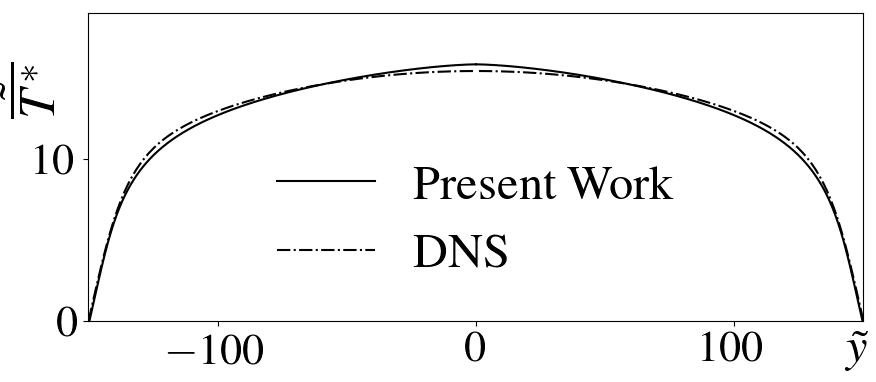
\includegraphics[angle=0, scale=0.24]{fotos_formatacao_final/Temperature_150_071_Prt(Ret)_Avelocity}
		\caption{Distribuição de temperatura para $Re_\tau = 150$, $L2 = 0.212$}
	\end{subfigure}
	\begin{subfigure}[t]{0.45\textwidth}
		\centering
		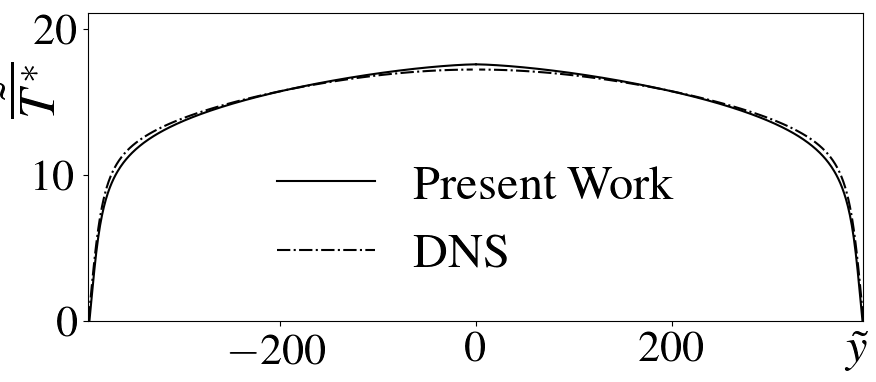
\includegraphics[angle=0, scale=0.24]{fotos_formatacao_final/Temperature_395_071_Prt(Ret)_Avelocity}
		\caption{Distribuição de temperatura para $Re_\tau = 395$, $L2 = 0.233$}
	\end{subfigure}
	\begin{subfigure}[t]{0.5\textwidth}
		\centering
		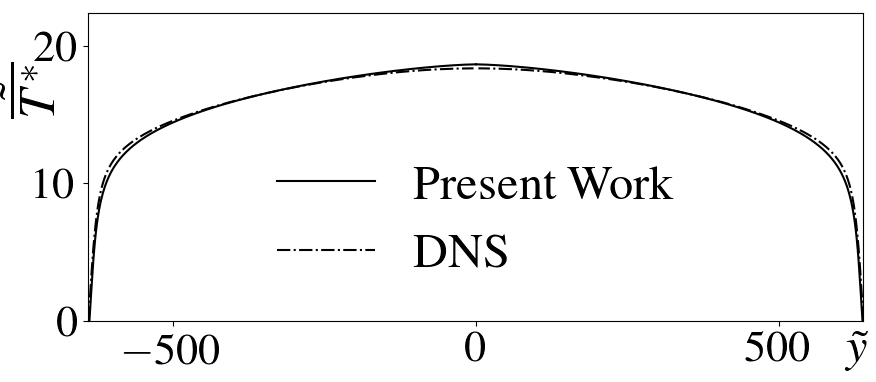
\includegraphics[angle=0, scale=0.24]{fotos_formatacao_final/Temperature_640_071_Prt(Ret)_Avelocity}
		\caption{Distribuição de temperatura para $Re_\tau = 640$, $L2 = 0.205$}
	\end{subfigure}
	\begin{subfigure}[t]{0.45\textwidth}
		\centering
		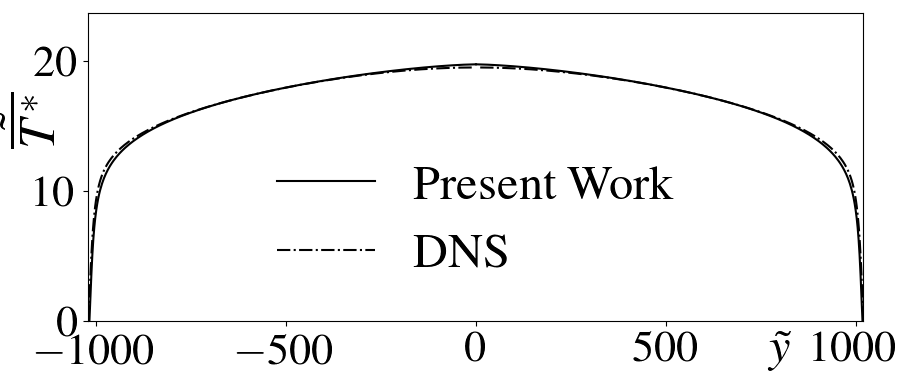
\includegraphics[angle=0, scale=0.24]{fotos_formatacao_final/Temperature_1000_071_Prt(Ret)_Avelocity}
		\caption{Distribuição de temperatura para $Re_\tau = 1020$, $L2 = 0.175$}
	\end{subfigure}	
	\caption{Resultado para simulações térmicas para $Pr_\tau(Re\tau)$, $A(Re_\tau)$ and $Pr =0.71$ }
\end{figure*}

Os valores do Cebeci que resultaram em um pequeno erro para o algoritmo da velocidade não tiveram o mesmo efeito nos resultados de temperatura. O Cebeci foi modelado para o erro de velocidade mínima, não sendo o melhor para a solução térmica. Algebricamente, a constante de Cebeci aparece duas vezes como se vê nas equações \ref{equationultima} e \ref{finalequationvelocity}. Então, é possível propor dois modelos de constantes de Cebeci. Um para a simulação dinâmica e outro para a simulação de temperatura.    


Outro método de ajuste na evolução diferencial é o ajuste multi objetivo. Tal abordagem foi usada para considerar mais de uma variável simultaneamente para otimização. Este método foi usado para ajustar a constante de Cebeci térmica e o número de Prandtl Turbulento para o menor erro (norma L2) no campo de temperatura resultante para cada amostra de DNS. A função dinâmica de Cebeci foi considerada a anteriormente desenvolvida. Novos valores ideais foram encontrados para o número de Prandtl turbulento e a constante térmica de Cebeci:

\begin{table}[!h]
	\centering
	\caption{Números de Prandtl turbulentos ideais e constantes de Cebeci ajustadas para cada número turbulento de Reynolds, com a abordagem multi objetiva. O Cebeci dinâmico continuou o mesmo da tabela \ref{tablea}. }
	\begin{tabular}{llll}
		\hline
		$Re_\tau$ & $Pr_t$ & $A_d$ & $A_v$\\
		\hline
		150  &   0.72530 & 37.25510 & 28.616180\\
		395  &   0.76821 & 34.24176 & 25.673782\\
		640  &   0.81896 & 31.27627 & 25.001266\\
		1020 &   0.86179 & 28.73726 & 25.002136\\ 
		\hline
	\end{tabular}
\end{table}
Com tais dados numéricos, foram propostos novos modelos para o número de Prandtl Turbulento e a constante térmica de Cebeci:

\begin{equation}
A_t = \frac{Re_\tau ^{0.0395059904287 \ln(Re_\tau)^2 - 0.758759596012 \ln(Re_\tau) +  4.66369525666  } }{e ^{5.67034263}}
\end{equation}

\begin{equation}
\begin{split}
Pr_t = -2.4891 * 10^{-10} Re_\tau^3 +  3.60362 * 10^{-7} Re_\tau^2 + 3.7921 *10 ^{-5} Re_\tau + 0.71234 
\end{split}
\end{equation}
Novas simulações foram desenvolvidas com essa parametrização:

\begin{figure*}[!h]
	\centering
	\begin{subfigure}[t]{0.5\textwidth}
		\centering
		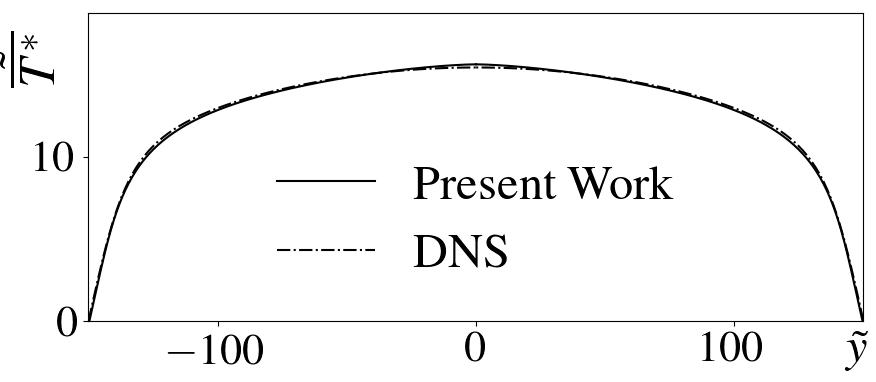
\includegraphics[angle=0, scale=0.24]{fotos_formatacao_final/Temperature_150_071_Genetic2temperature}
		\caption{Distribuição de temperatura para $Re_\tau = 150$, $L2 = 0.091$}
	\end{subfigure}
	\begin{subfigure}[t]{0.45\textwidth}
		\centering
		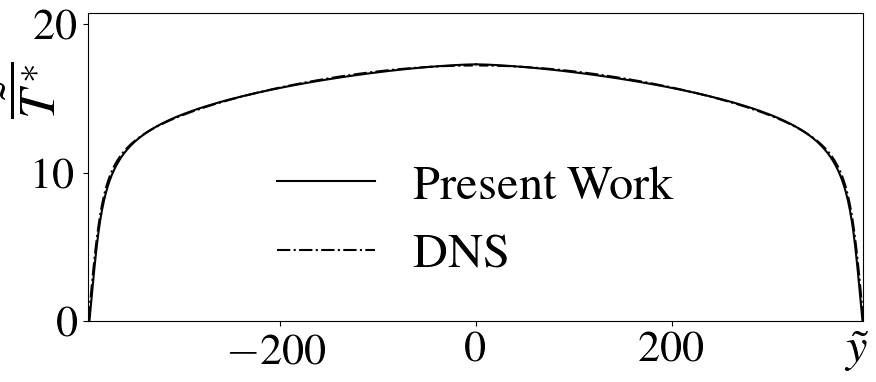
\includegraphics[angle=0, scale=0.24]{fotos_formatacao_final/Temperature_395_071_Genetic2temperature}
		\caption{Distribuição de temperatura para $Re_\tau = 395$, $L2 = 0.049$}
	\end{subfigure}
	\begin{subfigure}[t]{0.5\textwidth}
		\centering
		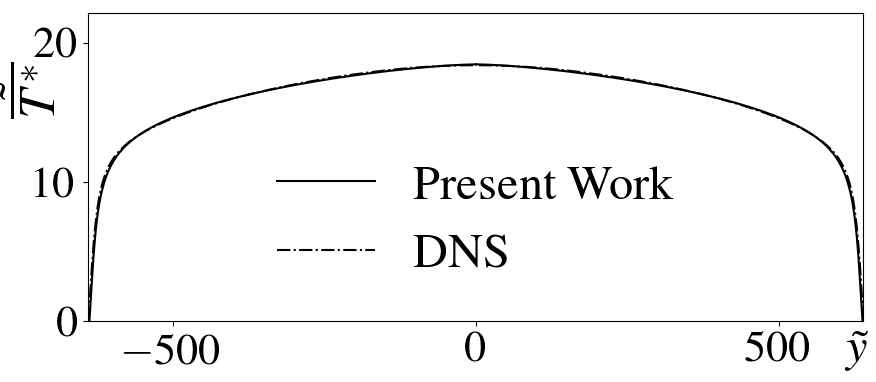
\includegraphics[angle=0, scale=0.24]{fotos_formatacao_final/Temperature_640_071_Genetic2temperature}
		\caption{Distribuição de temperatura para $Re_\tau = 640$, $L2 = 0.061$}
	\end{subfigure}
	\begin{subfigure}[t]{0.45\textwidth}
		\centering
		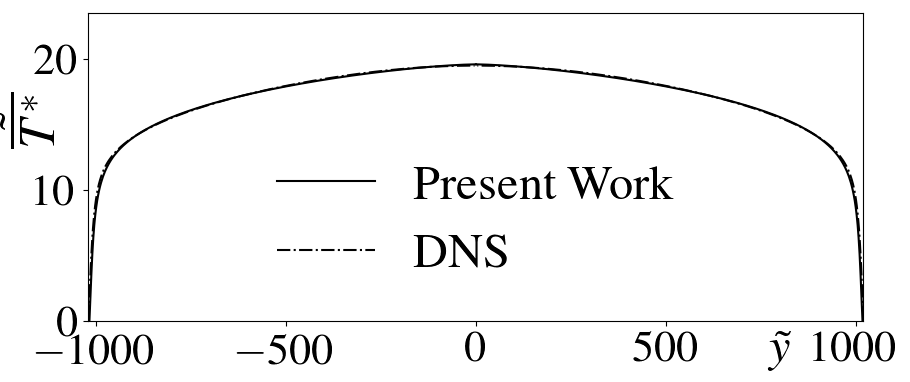
\includegraphics[angle=0, scale=0.24]{fotos_formatacao_final/Temperature_1000_071_Genetic2temperature}
		\caption{Distribuição de temperatura para $Re_\tau = 1020$, $L2 = 0.076$}
	\end{subfigure}	
	\caption{Resultados de simulações térmicas para $Pr_\tau(Re_\tau)$, $A_d(Re_\tau)$, $A_t(Re_\tau) $ e $Pr =0.71$, com ajuste multi objetivo.}
	\vspace{-5mm}
\end{figure*}



\chapter{Discussão}


\section{Resultados}

Com esses métodos, foram estudadas as vantagens e desvantagens de cada um. Uma comparação entre seus erros pode ser vista adiante:\\

\begin{figure}[!h]
	\centering
	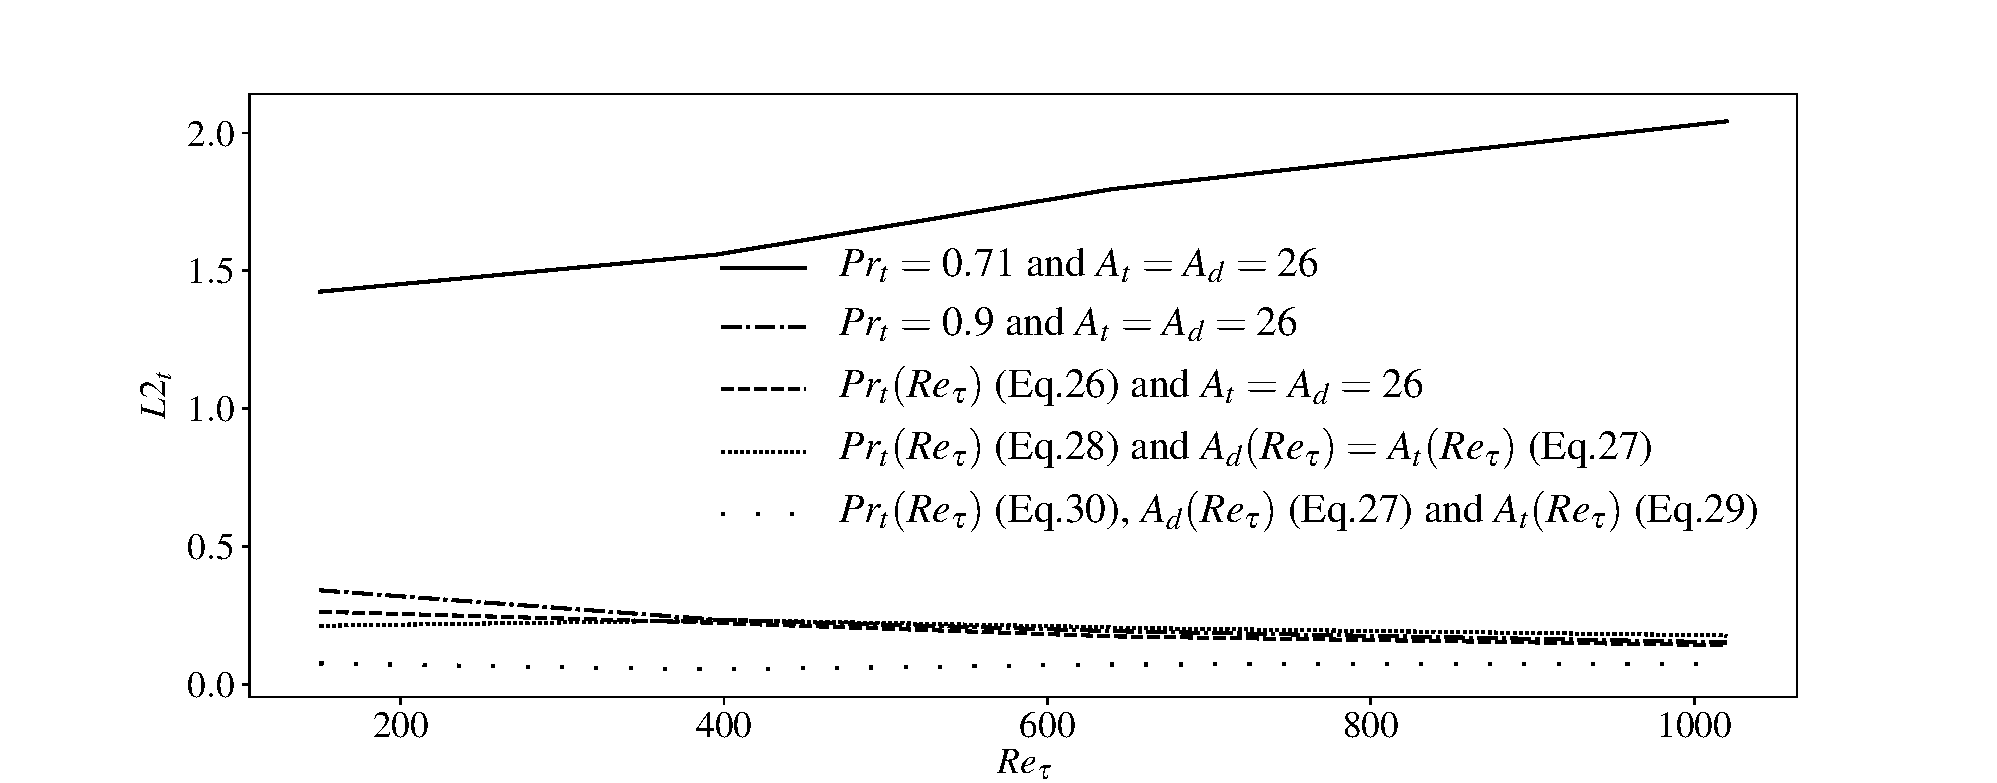
\includegraphics[angle=0, trim = {0mm 0mm 0mm 10mm}, scale=0.5]{fotos_formatacao_final/gerais}
	\caption{Comparison between all parameterizations for $Re_\tau$ and $Pr_t$.}
\end{figure}

Todos os modelos desenvolvidos no presente trabalho apresentaram melhores resultados que a parametrização clássica de $ Pr_t = 0.71 $ e $ A = 26 $ no escoamento turbulento de Poiseuille. A correção na constante do Cebeci, apesar de representar um erro menor na velocidade, não resultou em erros menores no perfil de temperatura para todo o domínio. O modelo que obteve os melhores resultados foi o desenvolvido com o algoritmo de evolução diferencial multi-objetivo em que foram considerados dois valores de Cebeci para cada domínio (térmico e dinâmico).

\section{Conclusões}

No presente trabalho foi desenvolvido com sucesso uma metodologia semi-analítica para calcular o perfil de temperatura em um canal com o modelo de comprimento de mistura Prandtl, um modelo clássico de fechamento no estudo da turbulência. As validações com o DNS foram satisfatórias. É importante notar que tais valores do número de Prandtl turbulento e constante de Cebeci foram aplicados para este caso particular, pois as parametrizações foram ajustes computacionais particulares e são simplificações das abstrações físicas que cada problema representa. Mas eles se adaptaram bem a este caso, resultando em precisão e eficiência. O método semi analítico foi bem sucedido no modelo do problema, pois bons resultados foram obtidos quando utilizados os números de Prandtl turbulento do DNS. Quanto aos modelos propostos, é uma ideia o aplicar então em outros problemas, com outras geometrias, como forma de testar sua universalidade.